\begin{figure}[!t]
\centering
\resizebox{\columnwidth}{!}{%
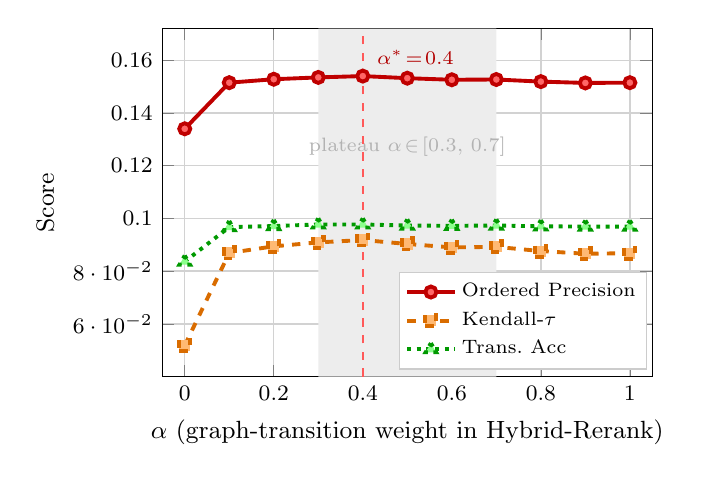
\begin{tikzpicture}
\begin{axis}[
  xlabel={$\alpha$ (graph-transition weight in Hybrid-Rerank)},
  ylabel={Score},
  xlabel style={font=\small},
  ylabel style={font=\small},
  tick label style={font=\footnotesize},
  xmin=-0.05, xmax=1.05,
  ymin=0.040, ymax=0.172,
  xtick={0,0.2,0.4,0.6,0.8,1.0},
  ytick={0.06,0.08,0.10,0.12,0.14,0.16},
  xticklabel style={font=\footnotesize},
  yticklabel style={font=\footnotesize},
  width=7.8cm, height=6.0cm,
  %% Legend: vertical, bottom-right, below all three lines
  legend style={font=\scriptsize, at={(0.99,0.02)}, anchor=south east,
    row sep=0pt, inner sep=2pt, draw=gray!40},
  legend cell align=left,
  grid=both,
  grid style={gray!20, line width=0.4pt},
  major grid style={gray!35, line width=0.5pt},
  clip=false,
]

%% ── Shaded plateau (0.3–0.7) ────────────────────────────────────────────────
\addplot[draw=none, fill=gray!14, forget plot]
  coordinates {(0.3,0.040)(0.7,0.040)(0.7,0.172)(0.3,0.172)} \closedcycle;

%% Plateau label at the TOP of the shaded band — above all data lines
\node[font=\scriptsize, text=gray!60, anchor=south]
  at (axis cs:0.5, 0.12)
  {plateau $\alpha\!\in\![0.3,\,0.7]$};

%% ── Ordered Precision ────────────────────────────────────────────────────────
\addplot[color=red!75!black, mark=*, mark size=2.0pt,
         line width=1.4pt, mark options={fill=red!60}]
  coordinates {
    (0.0, 0.134)
    (0.1, 0.1515)
    (0.2, 0.1528)
    (0.3, 0.1535)
    (0.4, 0.1540)
    (0.5, 0.1532)
    (0.6, 0.1526)
    (0.7, 0.1527)
    (0.8, 0.1519)
    (0.9, 0.1514)
    (1.0, 0.1515)
  };
\addlegendentry{Ordered Precision}

%% ── Kendall-τ ────────────────────────────────────────────────────────────────
\addplot[color=orange!85!black, mark=square*, mark size=2.0pt,
         line width=1.4pt, dashed, mark options={fill=orange!55}]
  coordinates {
    (0.0, 0.0518)
    (0.1, 0.0869)
    (0.2, 0.0894)
    (0.3, 0.0909)
    (0.4, 0.0918)
    (0.5, 0.0903)
    (0.6, 0.0890)
    (0.7, 0.0892)
    (0.8, 0.0876)
    (0.9, 0.0866)
    (1.0, 0.0868)
  };
\addlegendentry{Kendall-$\tau$}

%% ── Transition Accuracy ──────────────────────────────────────────────────────
\addplot[color=green!60!black, mark=triangle*, mark size=2.2pt,
         line width=1.4pt, dotted, mark options={fill=green!45}]
  coordinates {
    (0.0, 0.0836)
    (0.1, 0.0967)
    (0.2, 0.0971)
    (0.3, 0.0977)
    (0.4, 0.0977)
    (0.5, 0.0973)
    (0.6, 0.0972)
    (0.7, 0.0973)
    (0.8, 0.0970)
    (0.9, 0.0969)
    (1.0, 0.0969)
  };
\addlegendentry{Trans.~Acc}

%% ── Best-α marker — label placed to the RIGHT of the dashed line ─────────────
\draw[red!65, dashed, line width=0.7pt]
  (axis cs:0.4,0.040) -- (axis cs:0.4,0.172);
\node[font=\scriptsize, text=red!70!black, anchor=south west]
  at (axis cs:0.41, 0.1545) {$\alpha^*\!=\!0.4$};

\end{axis}
\end{tikzpicture}}%
\caption{$\alpha$ sensitivity of GS-Hybrid+Hybrid-Rerank on ToolBench
(Stage~1 fixed; Stage~2 Hybrid-Rerank weight varied).
All three metrics jump sharply from $\alpha{=}0$ (semantic only)
to $\alpha{=}0.1$ (graph added), then plateau over
$\alpha\!\in\![0.3,\,0.7]$, confirming that Stage~1 and Stage~2
can be optimised independently.}
\label{fig:alpha}
\end{figure}
